\section{Influence of other parameters}
\label{sec:8}

For every simulation of this paper, orbital parameters and asteroid properties are referenced in \autoref{sec:4.3}, excepted for comparison simulation in \autoref{fig:6.3} with two different obliquities and in \autoref{fig:7.2} with two different revolution periods. It might be essential to observe the change on the surface temperature when varying other parameters such as the thermal intertia and the heliocentric distance. The thermal camera needs and other tools on board rely on the changes in thermal inertia. Studying the evolution of the temperature with different heliocentric distances is important as the position of asteroids changes and especially Didymoon (from 1.1 AU to 1.9 AU). Juventas, a small satellite on board on the spacecraft Hera, and it has the mission to land on Didymoon to analyse the cratere post impact formed by the DART mission. The range of landing is around 1.7 AU and 1.9 AU, and expected thermal inertia is in the range of 50---500 \si{J.K^{-1}.m^{-2}.s^{-1/2}}.

\begin{figure*}[b]
    \centering
	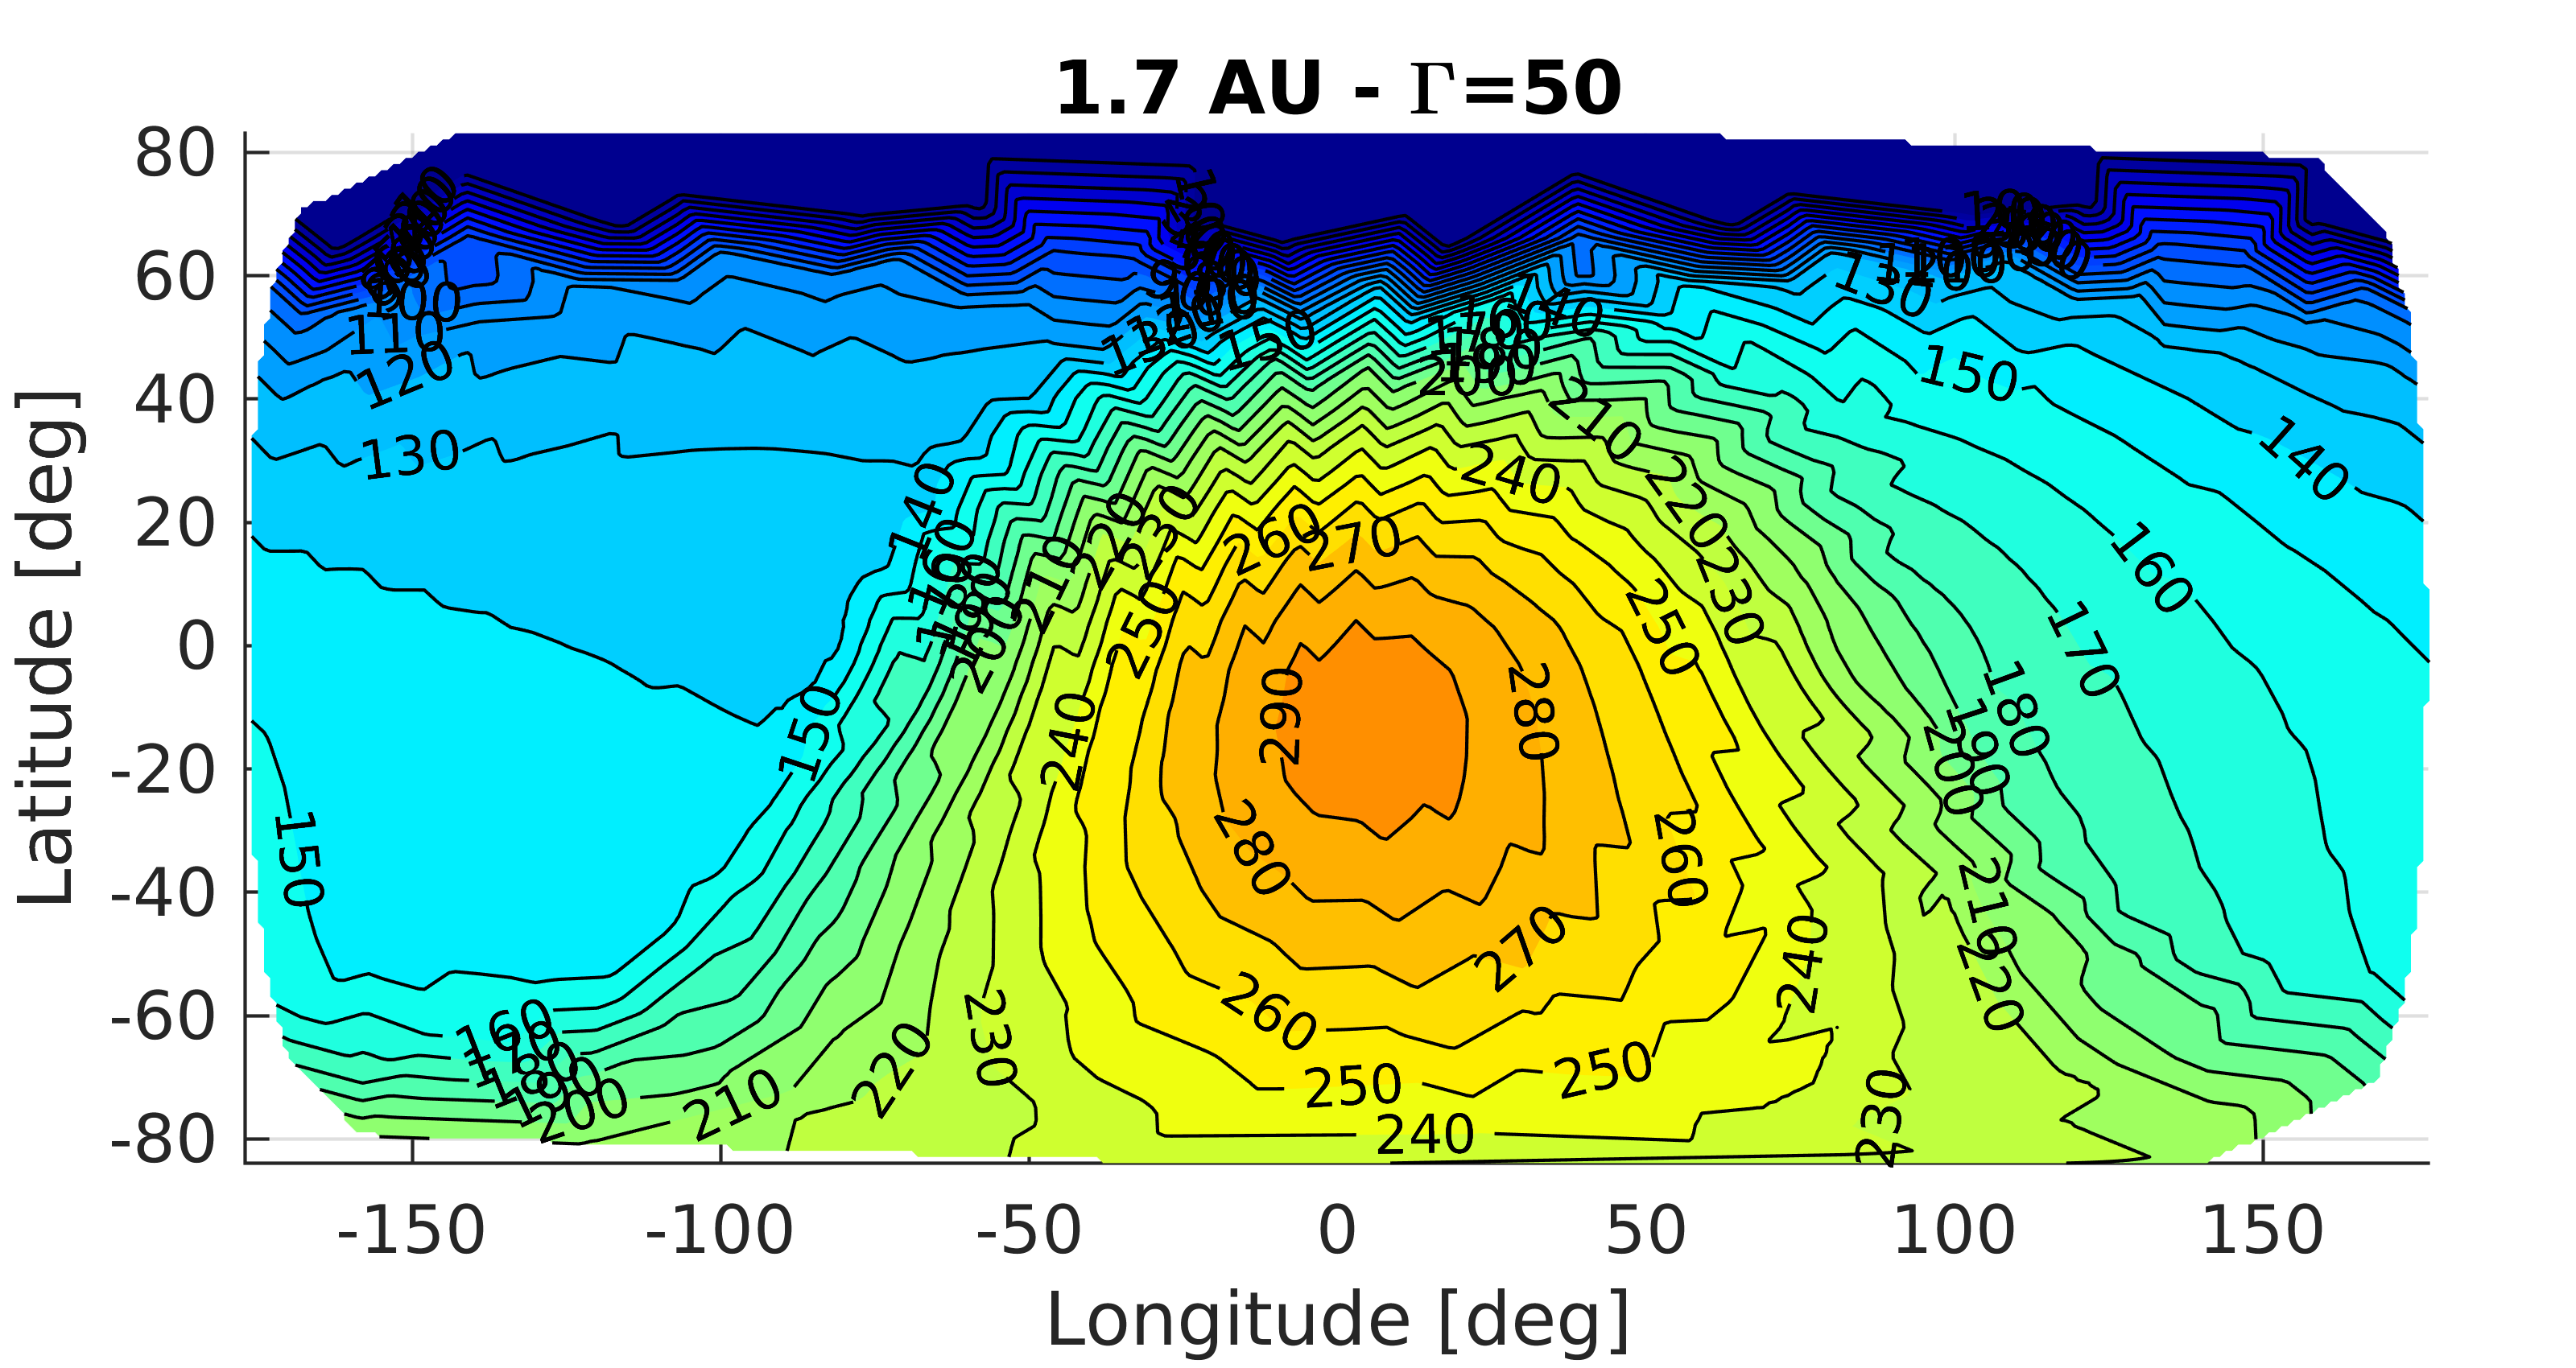
\includegraphics[width=0.3\linewidth]{rsc/juventas_d1,7_g50.png}
	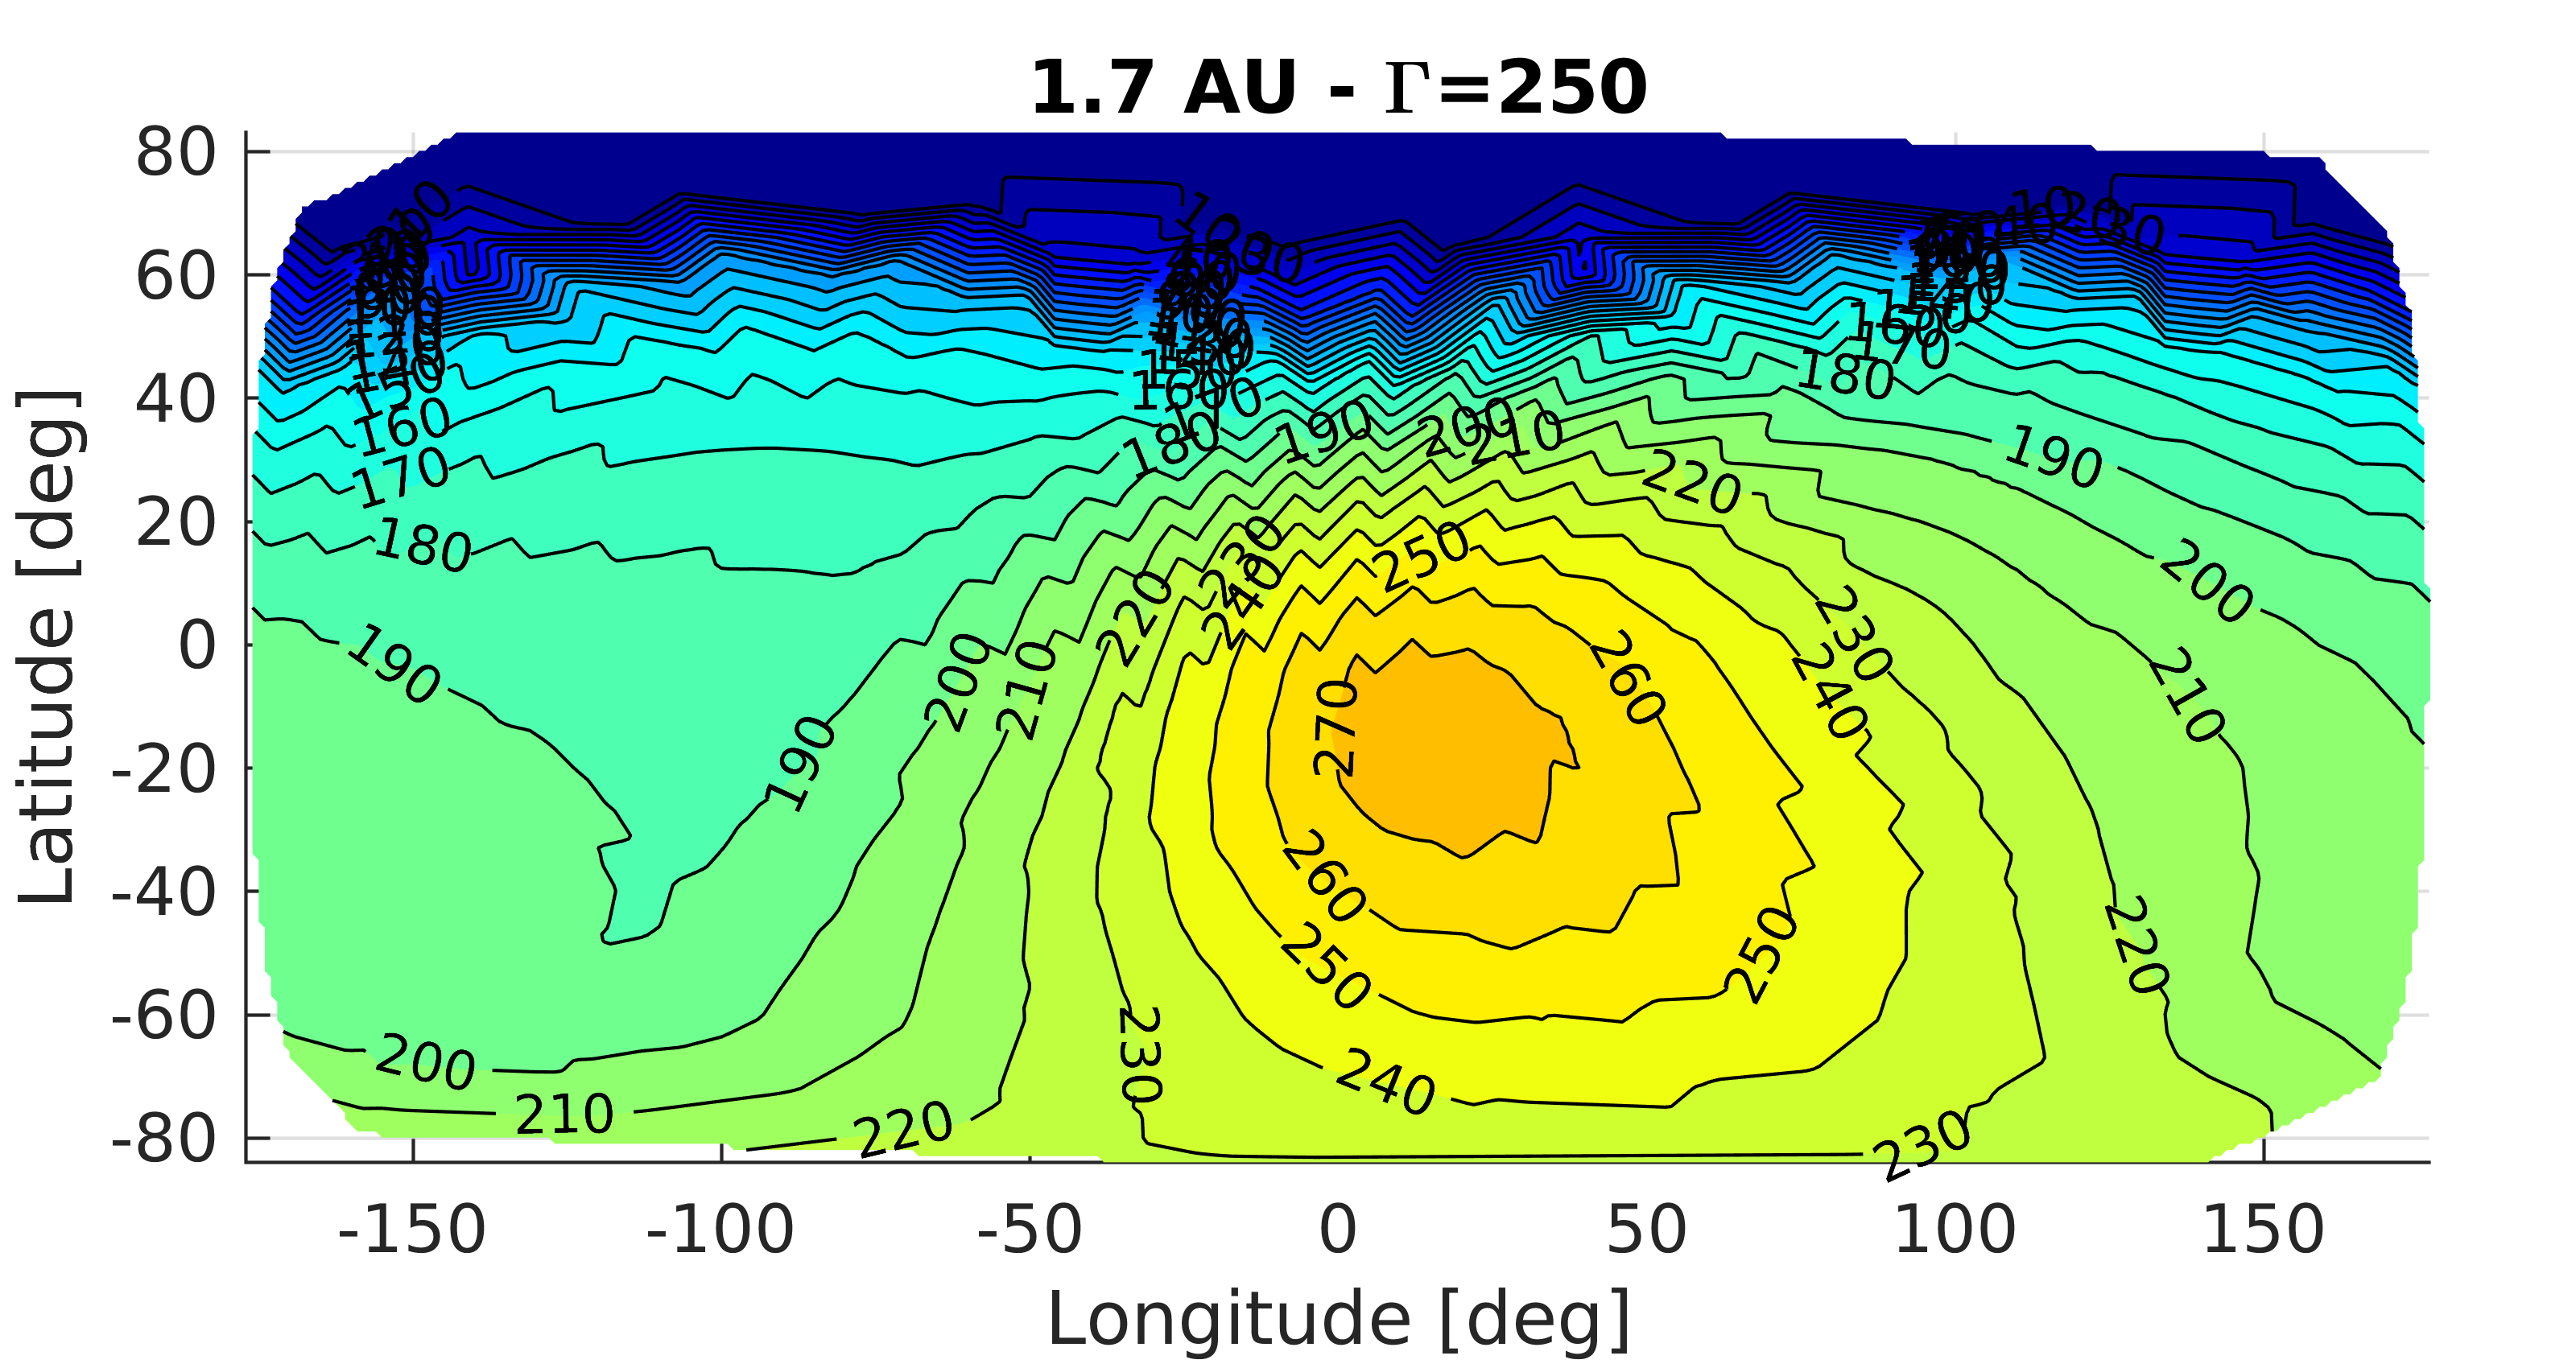
\includegraphics[width=0.3\linewidth]{rsc/juventas_d1,7_g250.png}
	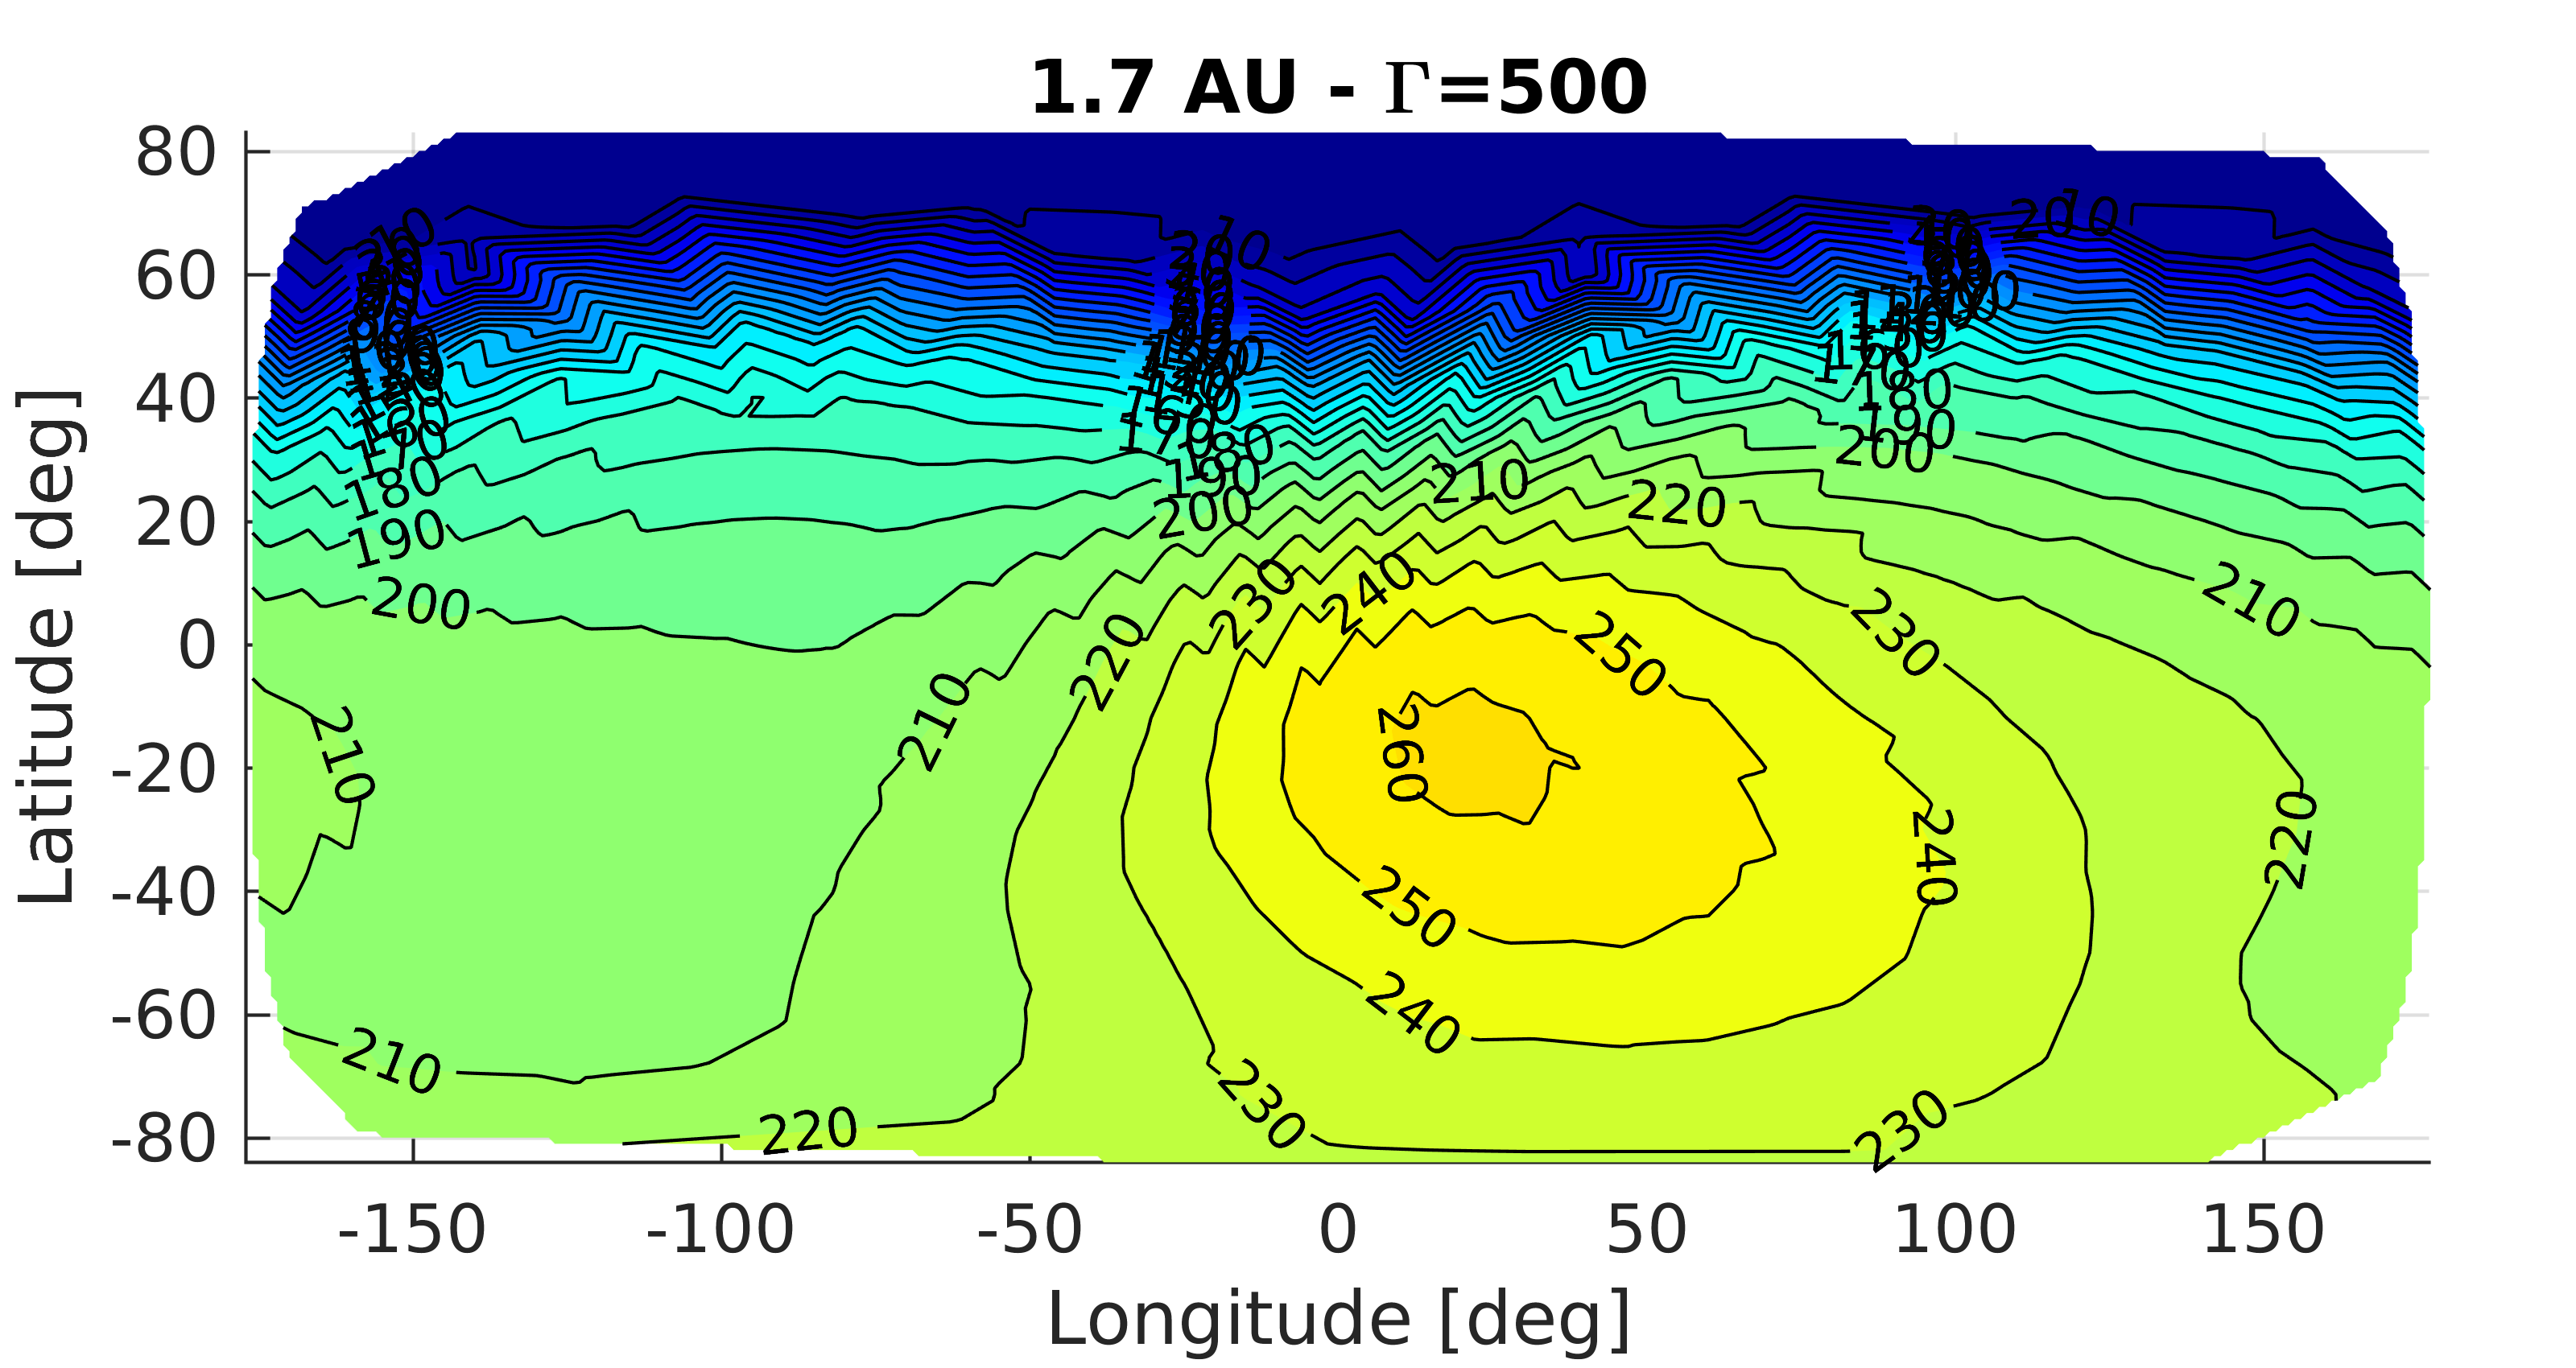
\includegraphics[width=0.3\linewidth]{rsc/juventas_d1,7_g500.png}\\
	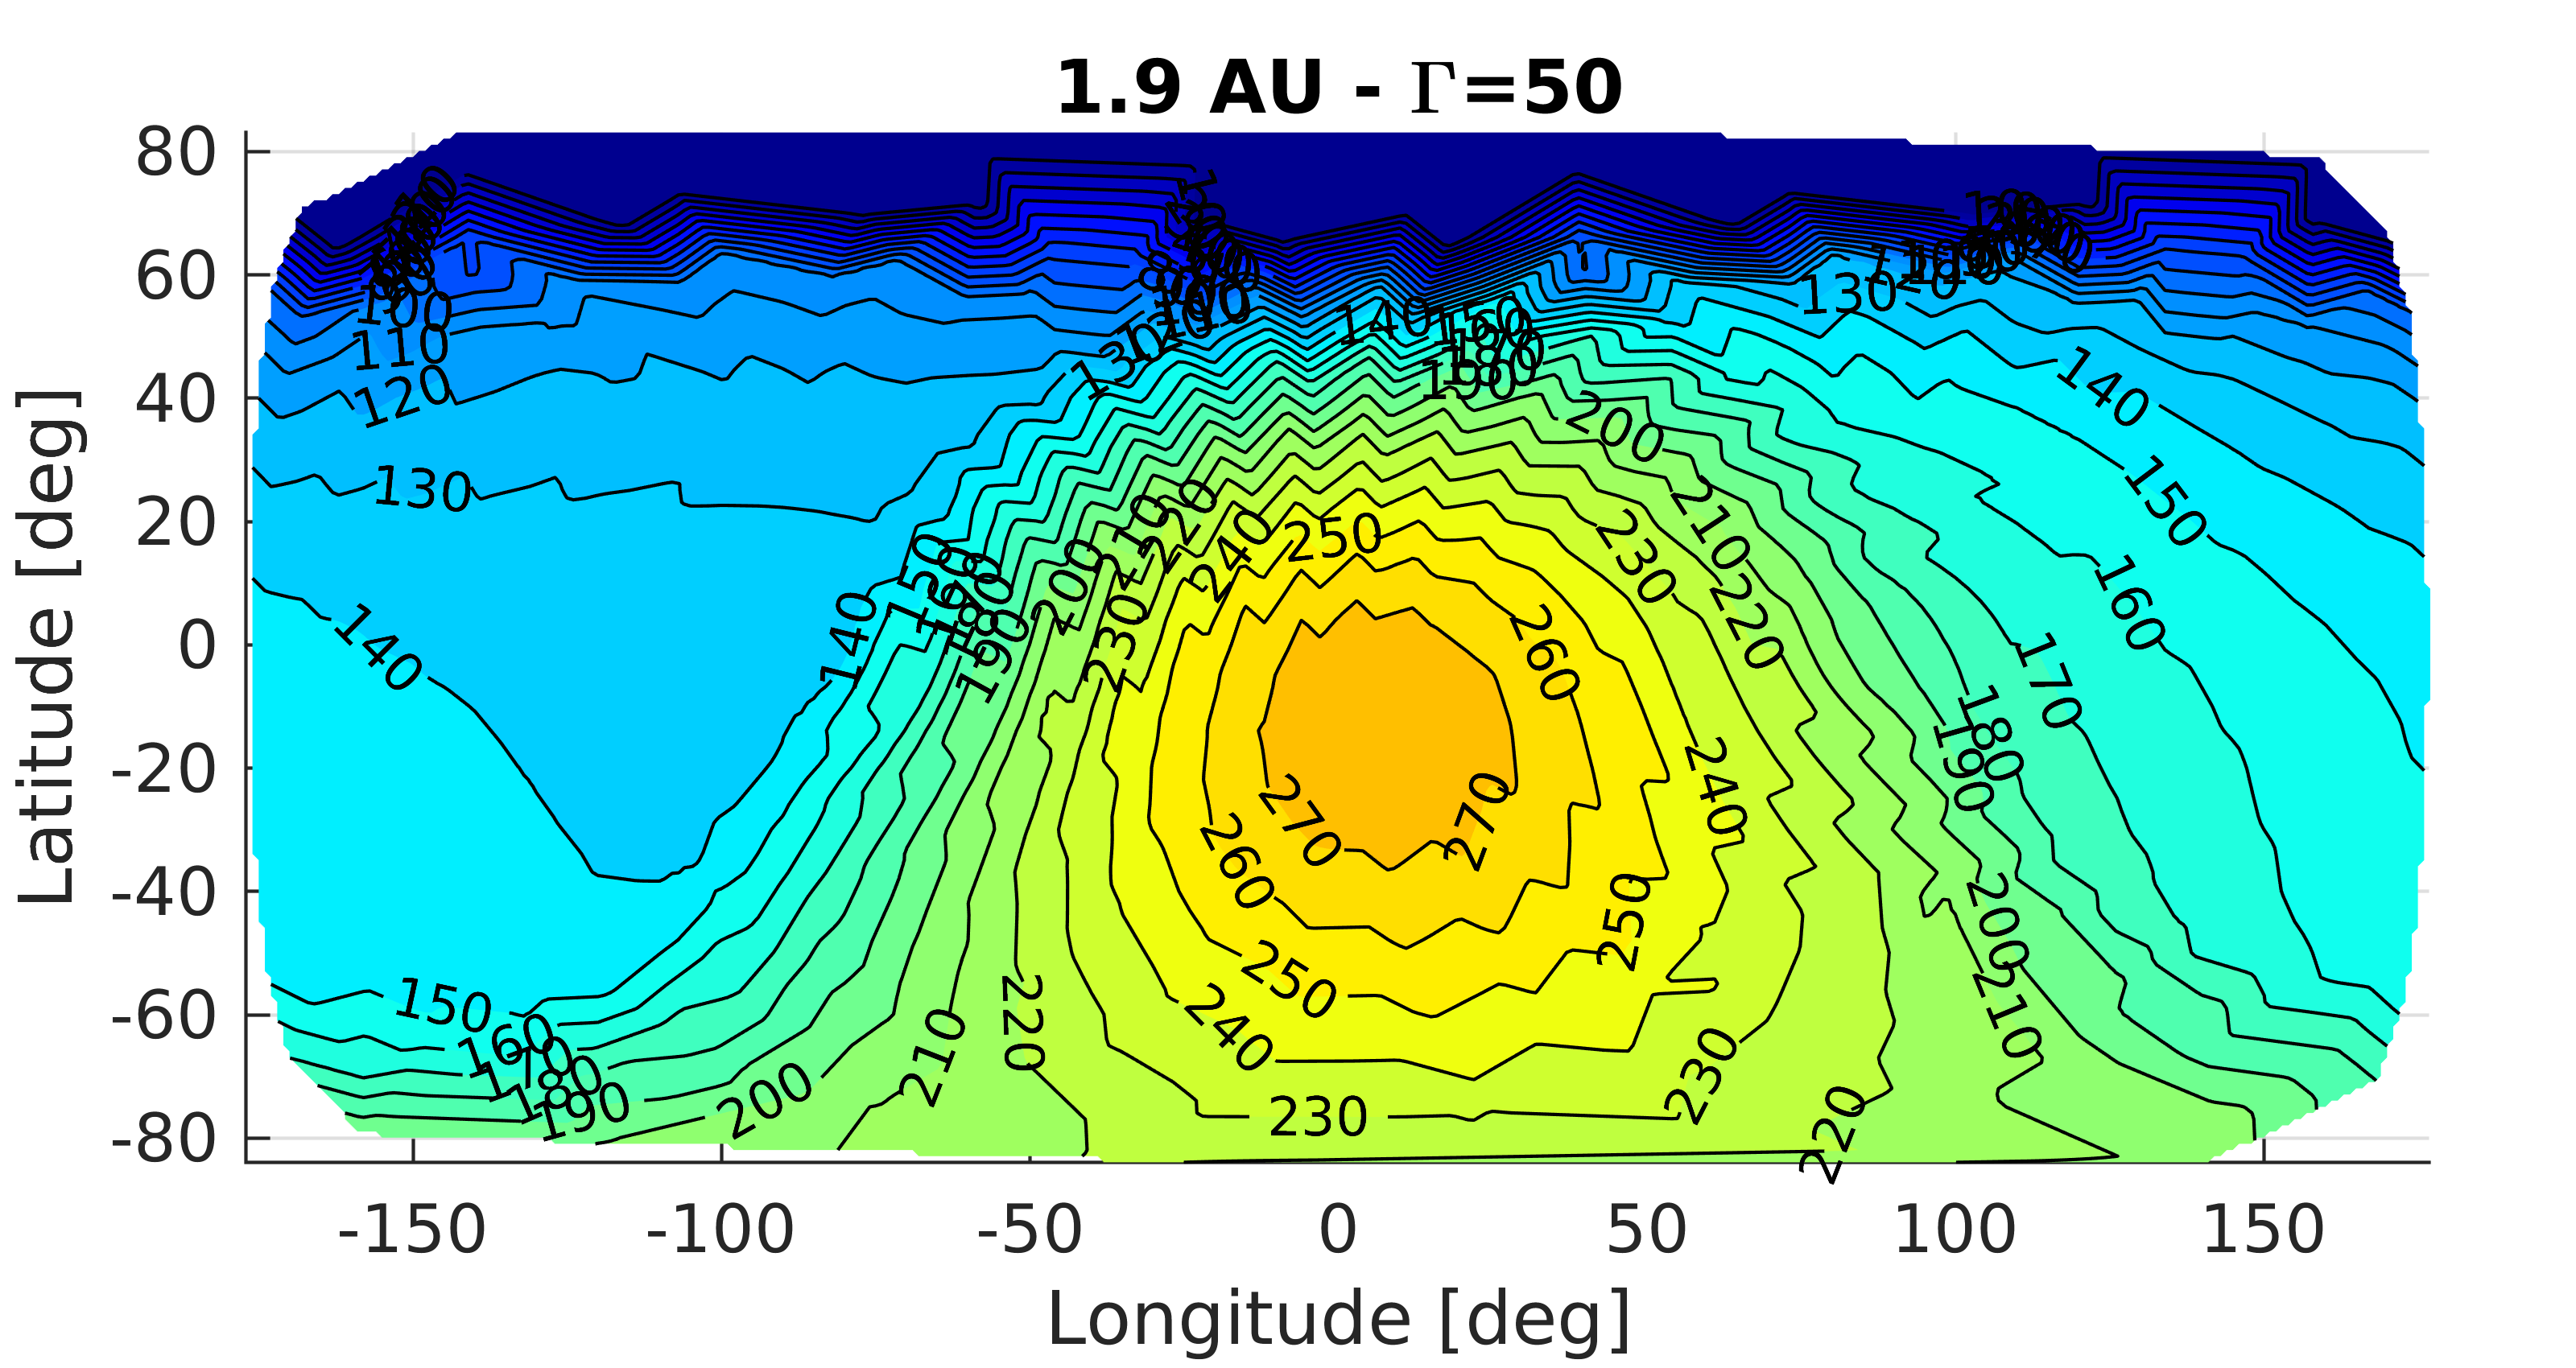
\includegraphics[width=0.3\linewidth]{rsc/juventas_d1,9_g50.png}
	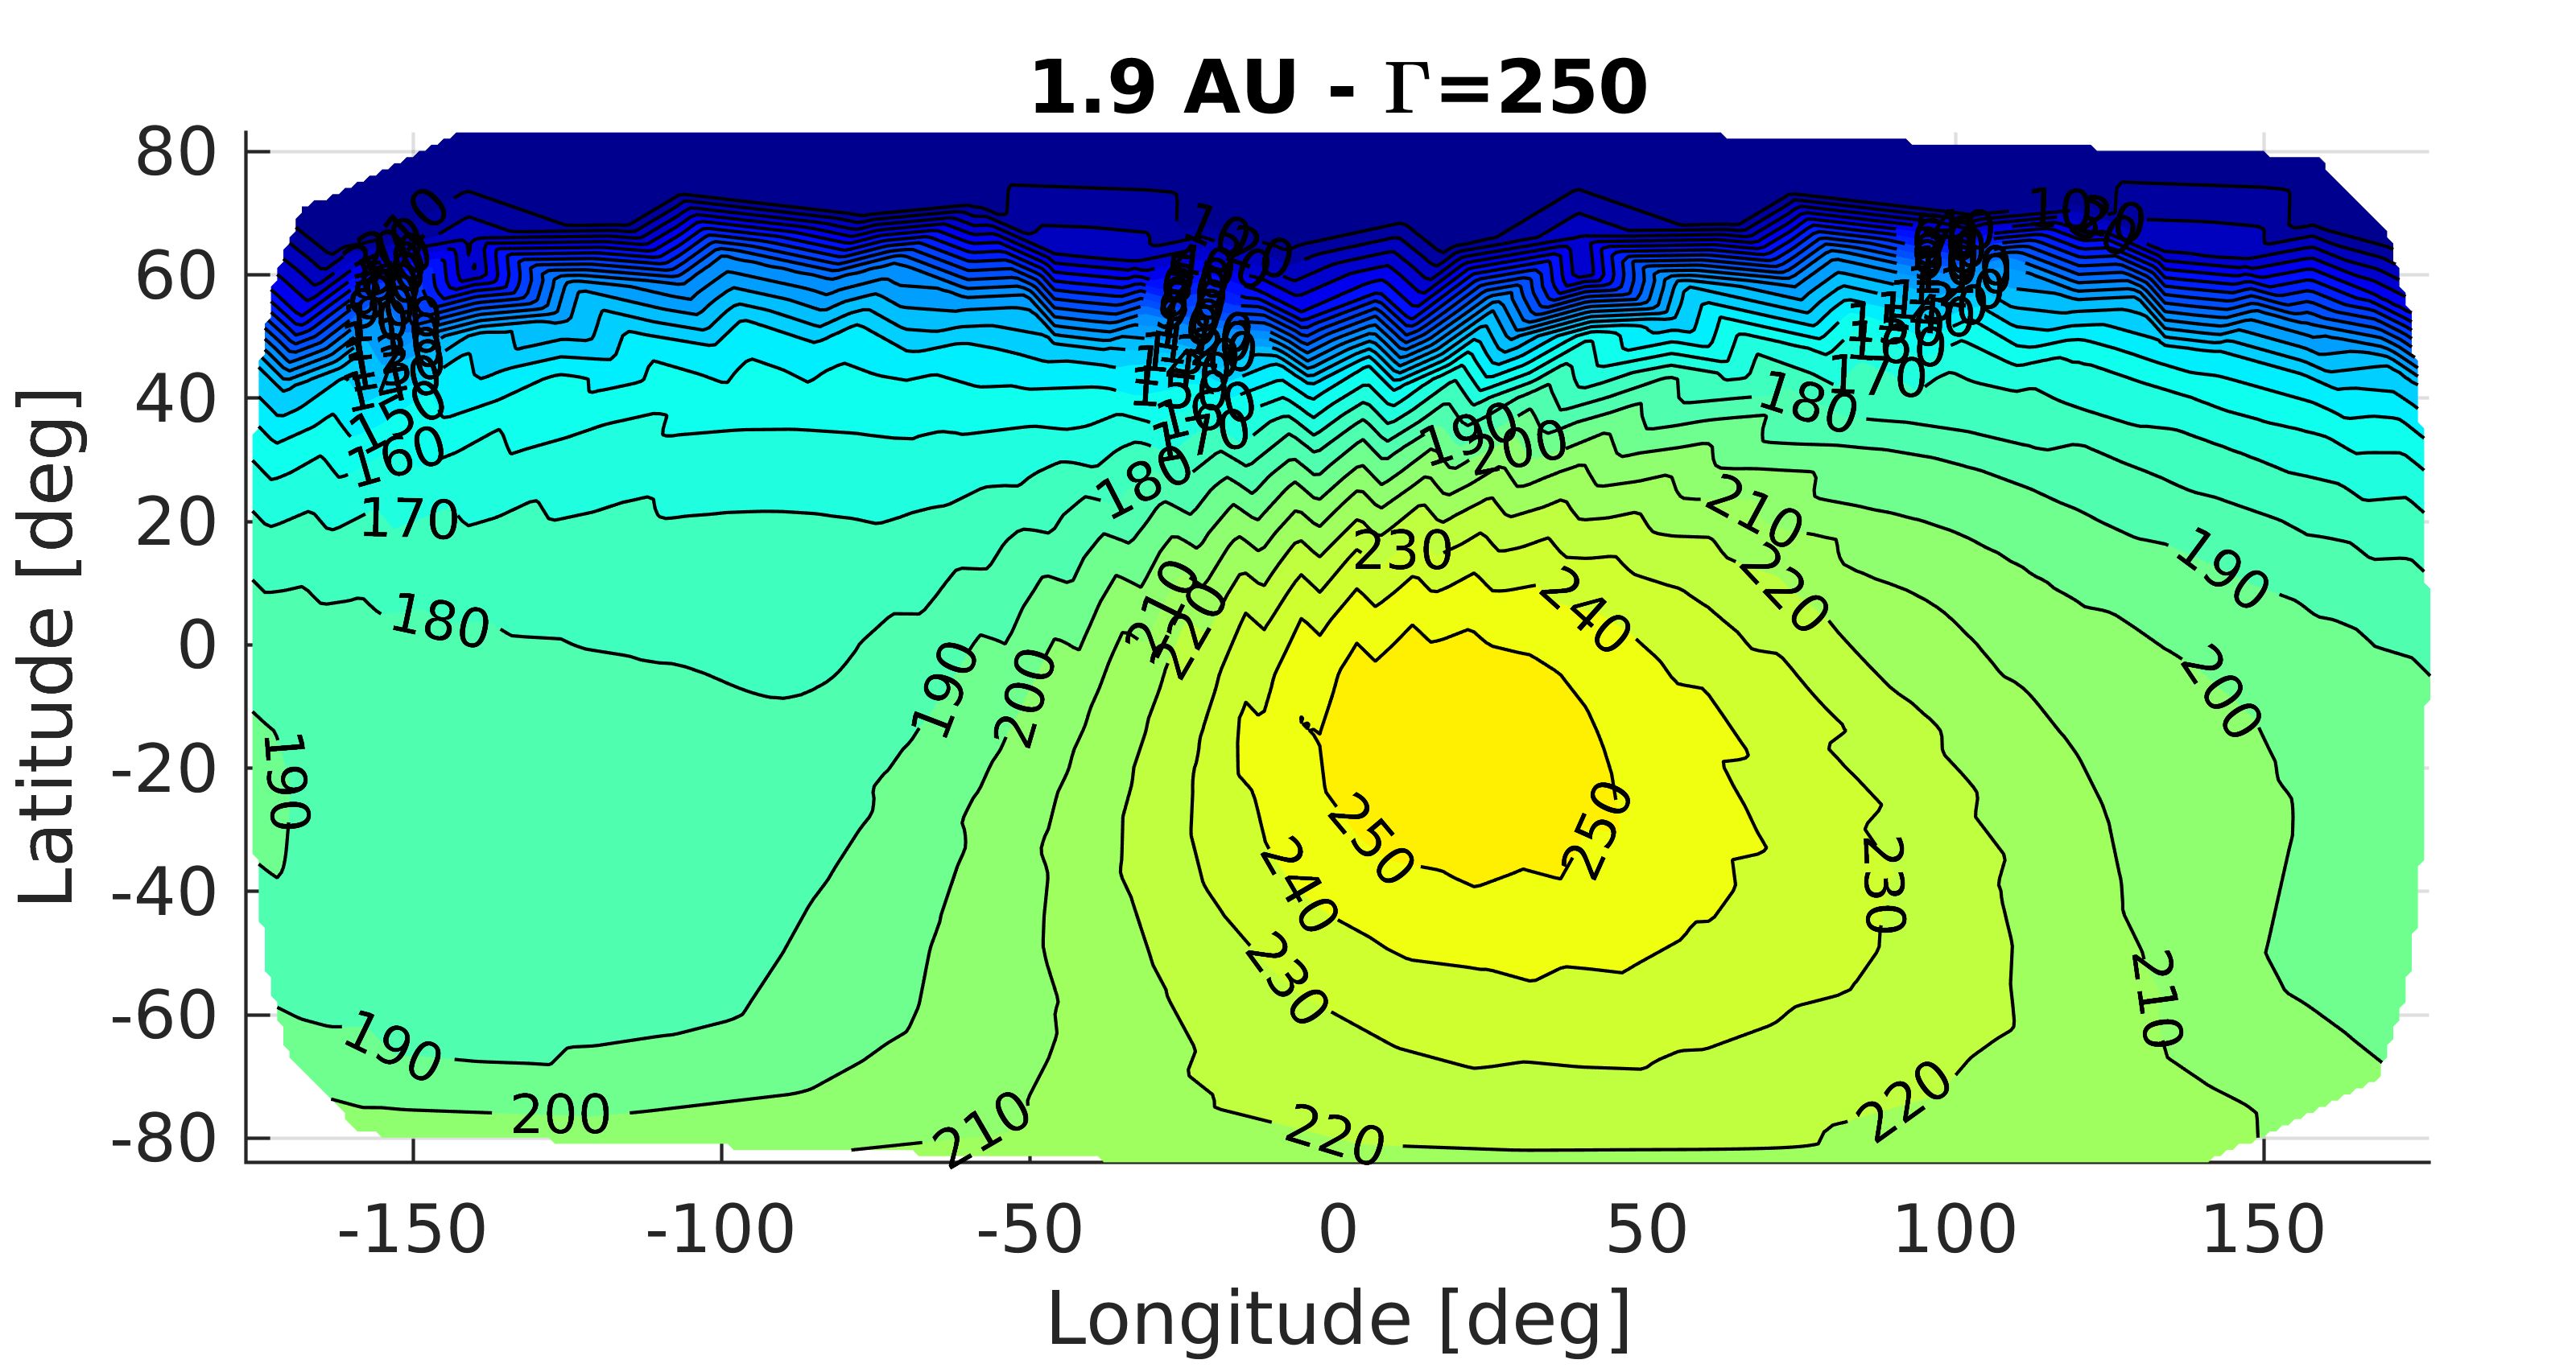
\includegraphics[width=0.3\linewidth]{rsc/juventas_d1,9_g250.png}
	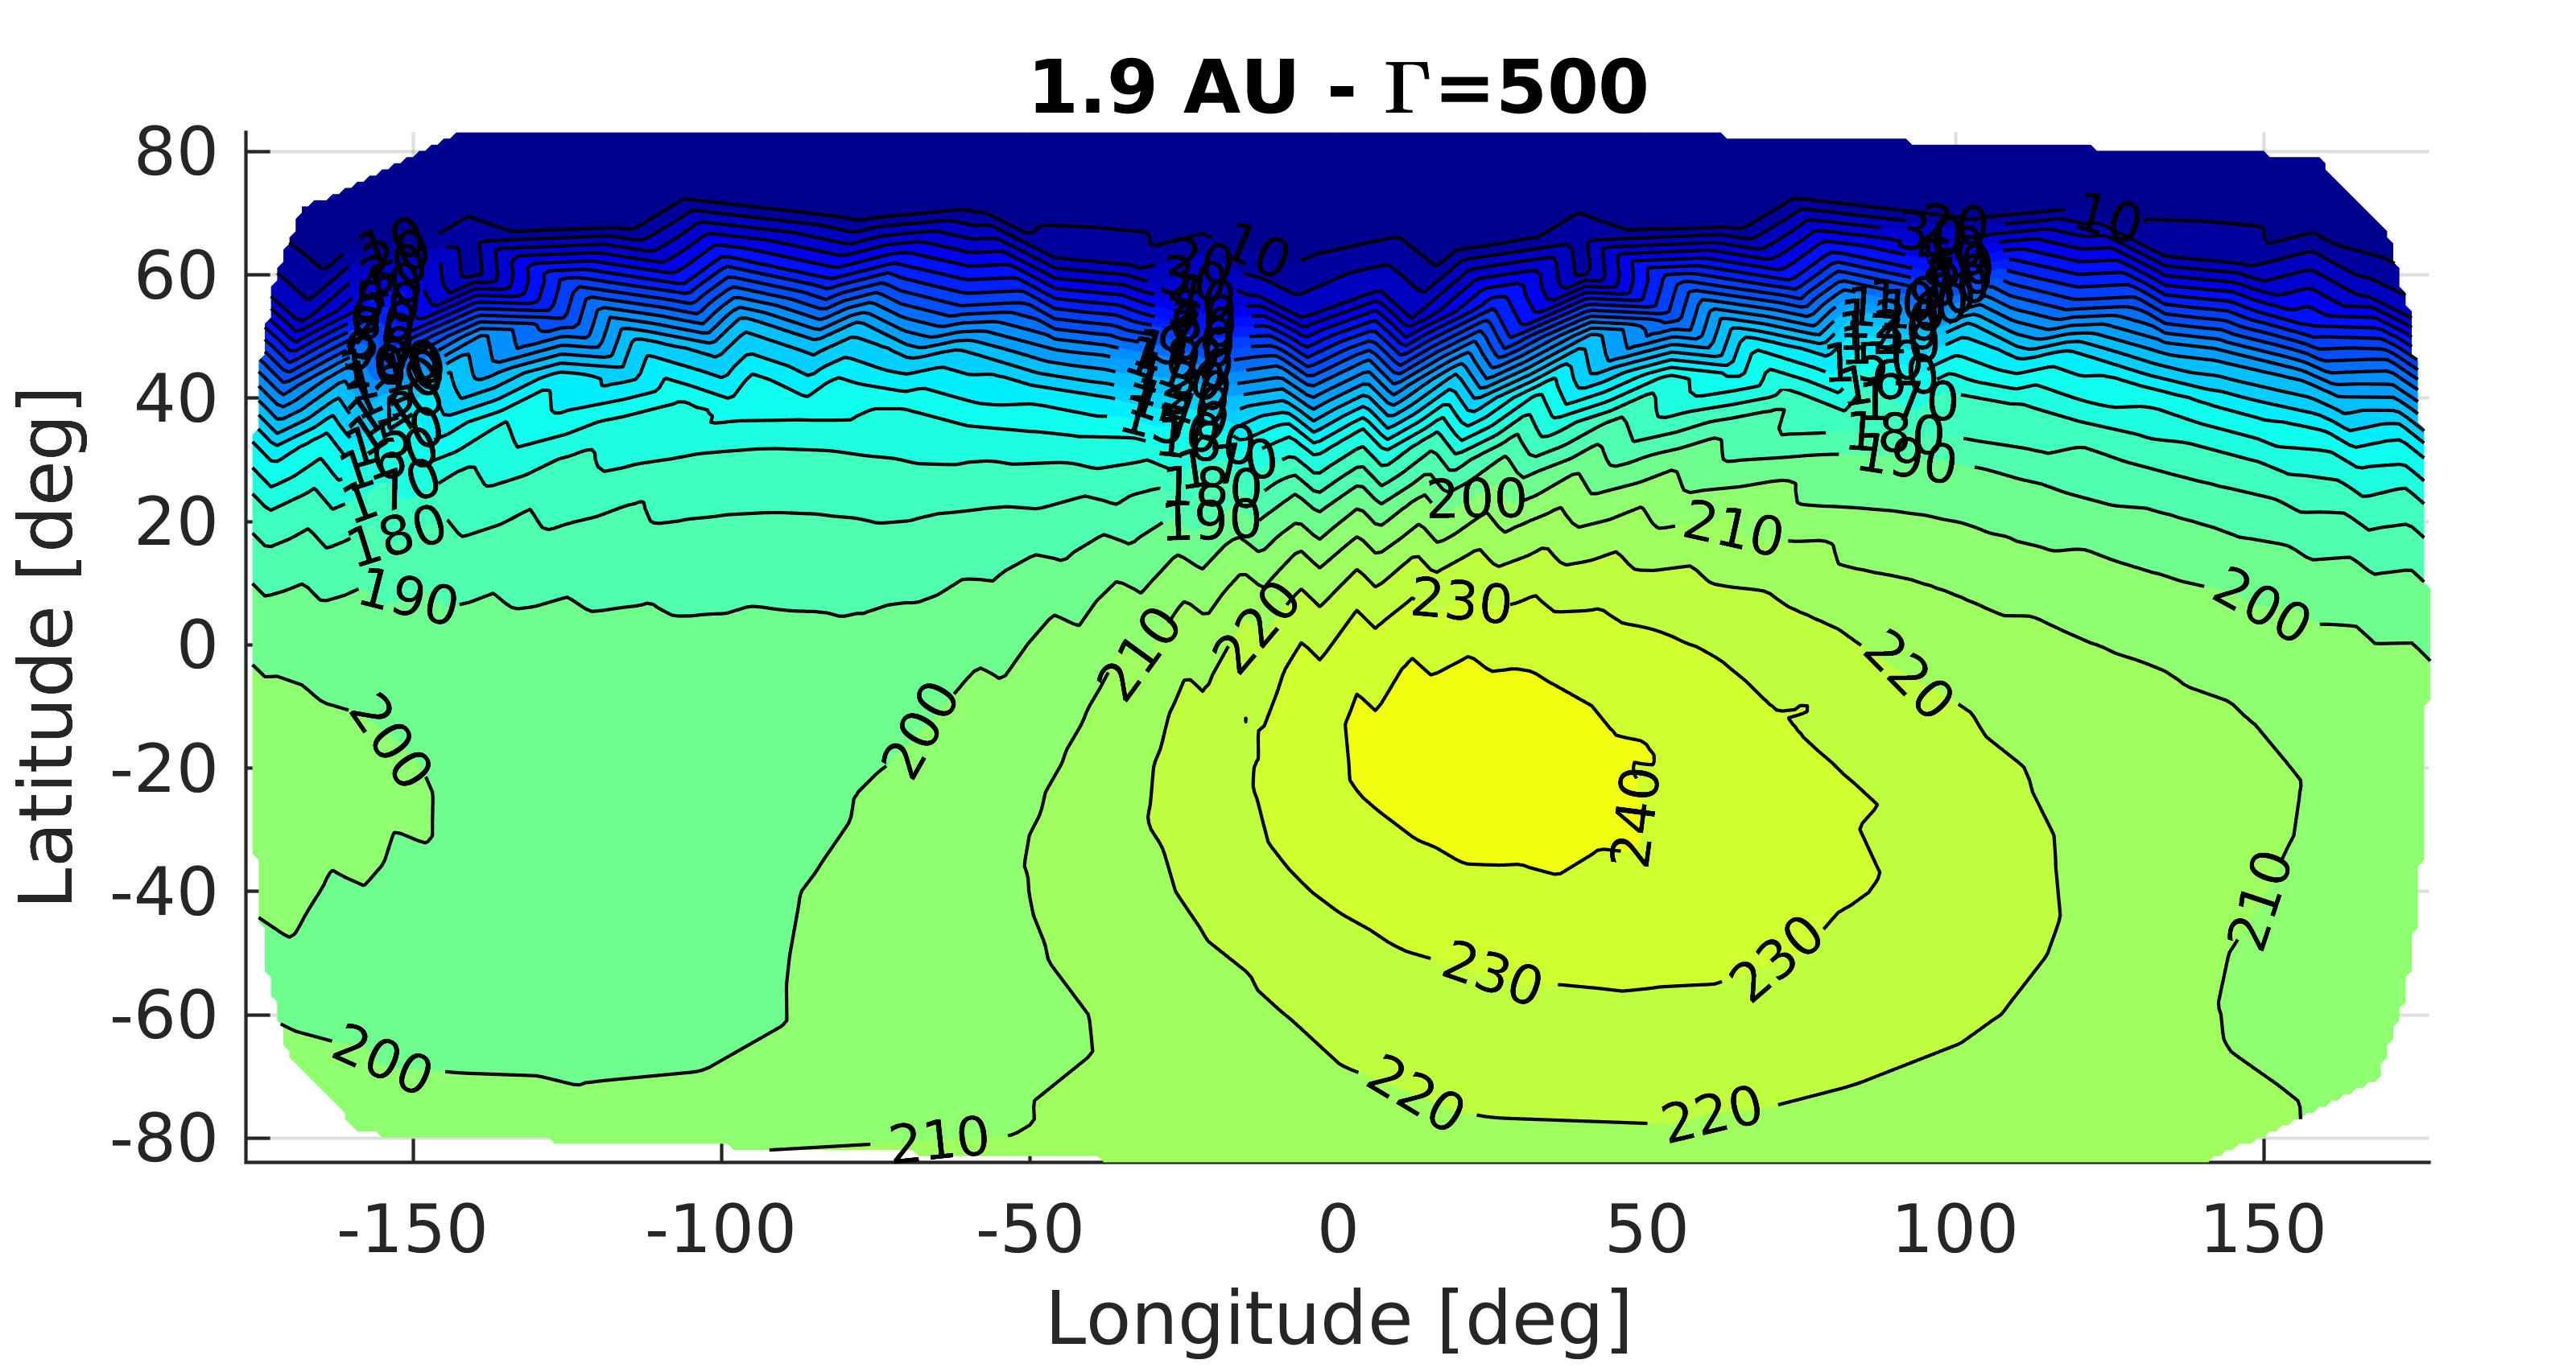
\includegraphics[width=0.3\linewidth]{rsc/juventas_d1,9_g500.png}
	\caption{Thermal map of the surface temperature on Didymoon for different thermal inertia and heliocentric distance.}
    \label{fig:8.1}
\end{figure*}

Results can be seen in \autoref{fig:8.1}. Variation of the thermal inertia impacts heat sensibility -- pretty much as variations of the revolution period seen in \autoref{sec:7}. The higher the thermal inertia, the lesser the heat sensitivity and the lesser the temperature varies. The impact of the distance on temperature was predicted.

Further works in the study of the influence of the thermal inertia on the surface temperature lead to \autoref{fig:8.2}
\begin{center}
    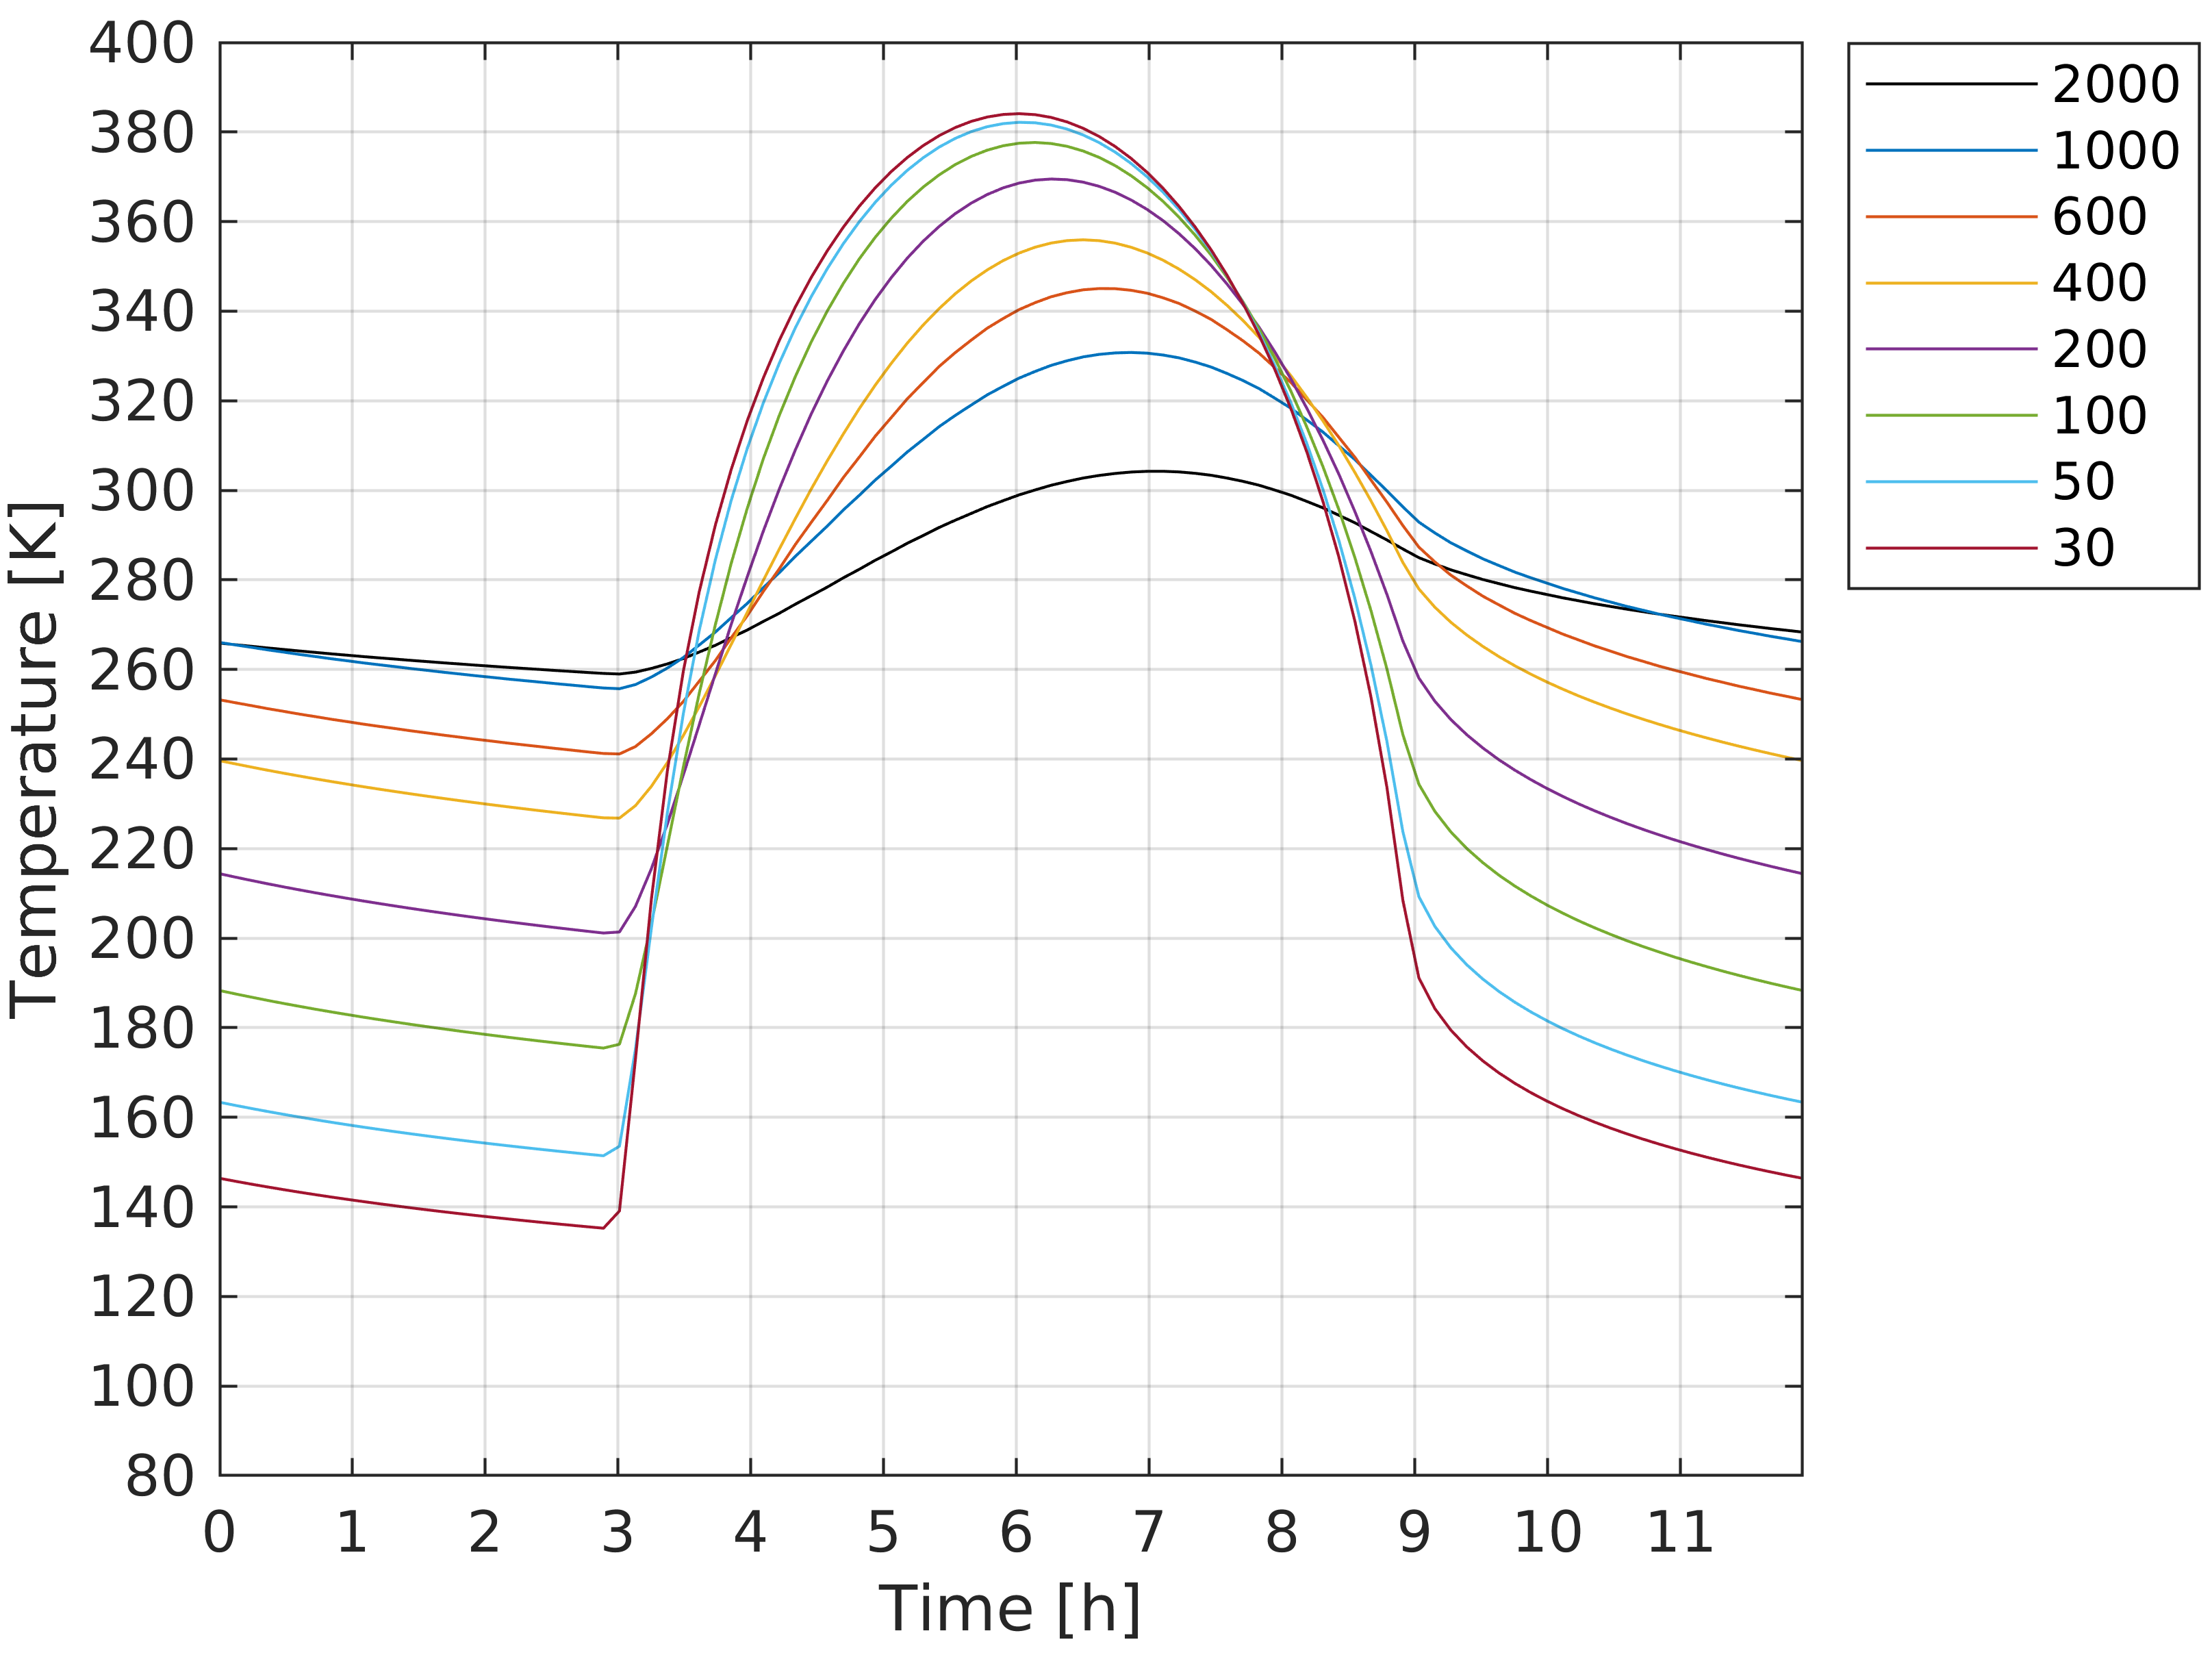
\includegraphics[width=\linewidth]{rsc/temp_r1,0501_gammas.png}
    \captionof{figure}{Influence of the thermal intertia on the daily surface temperatures. Simulation with an heliocentric distance of 1.0501 AU.}
    \label{fig:8.2}
\end{center}

When the thermal inertia varies, the maximum and minimum surface temperature values change, as presented in \autoref{fig:8.3}.
\begin{figure*}[t]
    \centering
    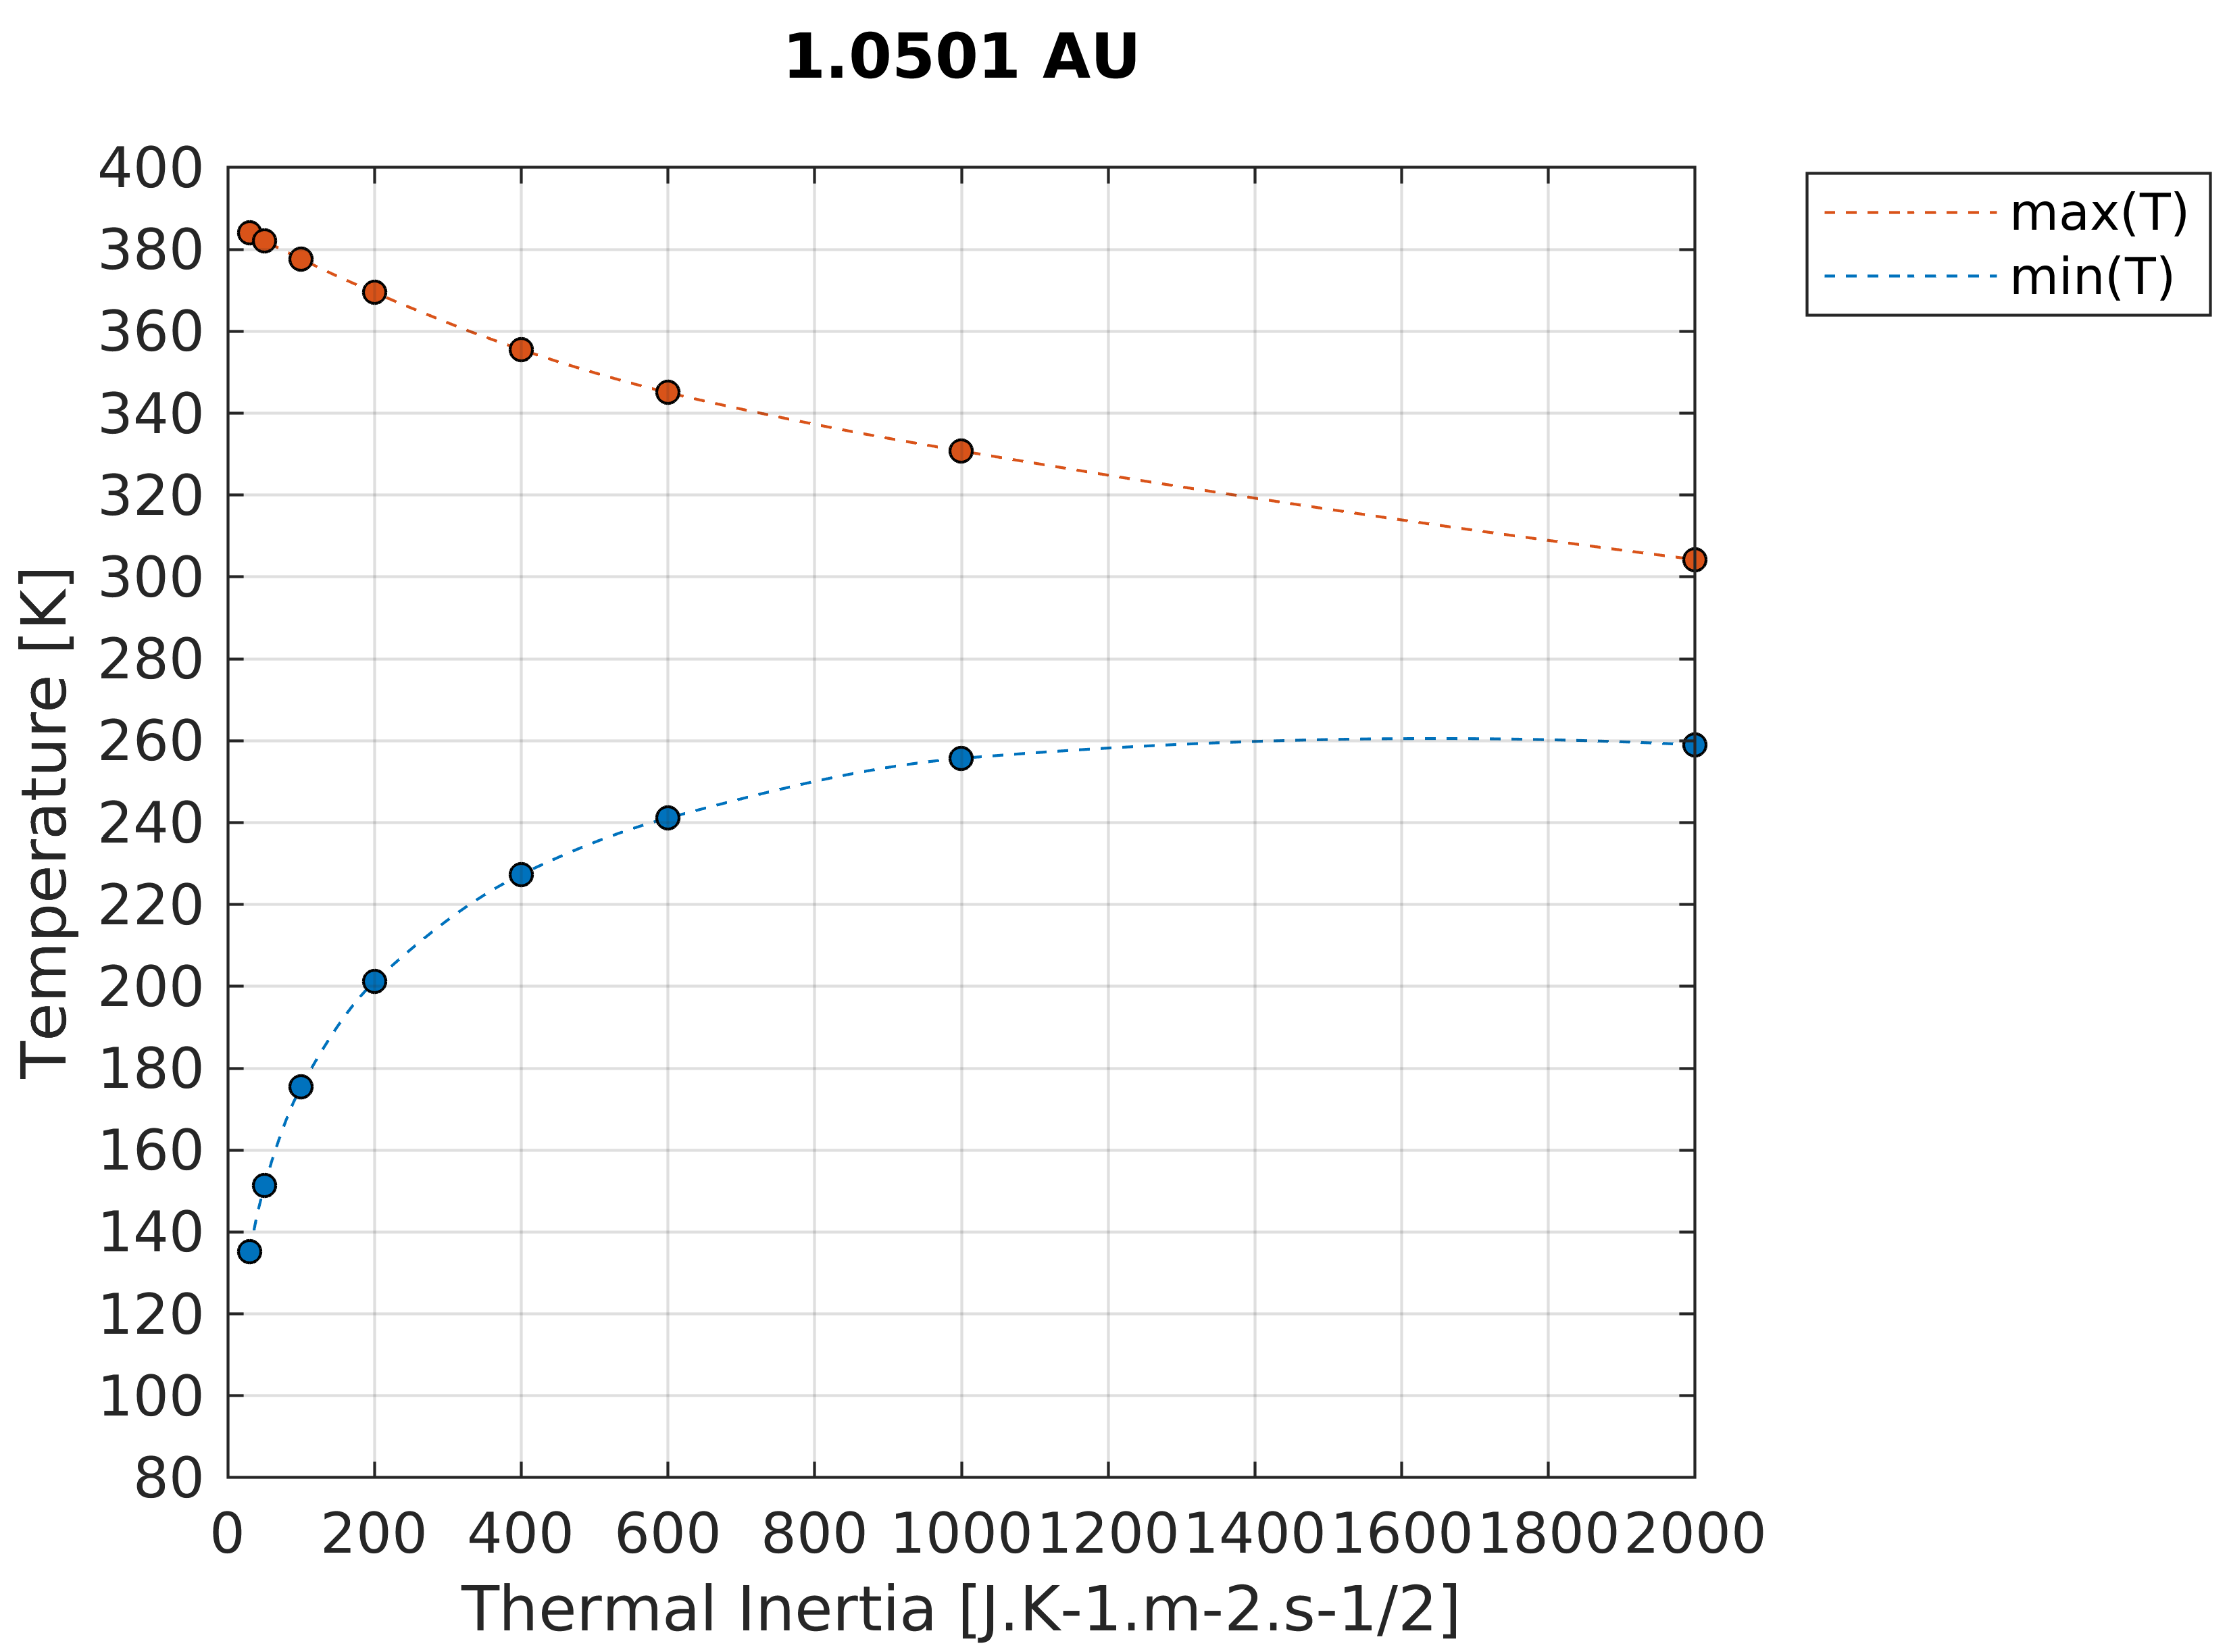
\includegraphics[width=0.49\linewidth]{rsc/temp_r1,0501_gammas_max.png}
    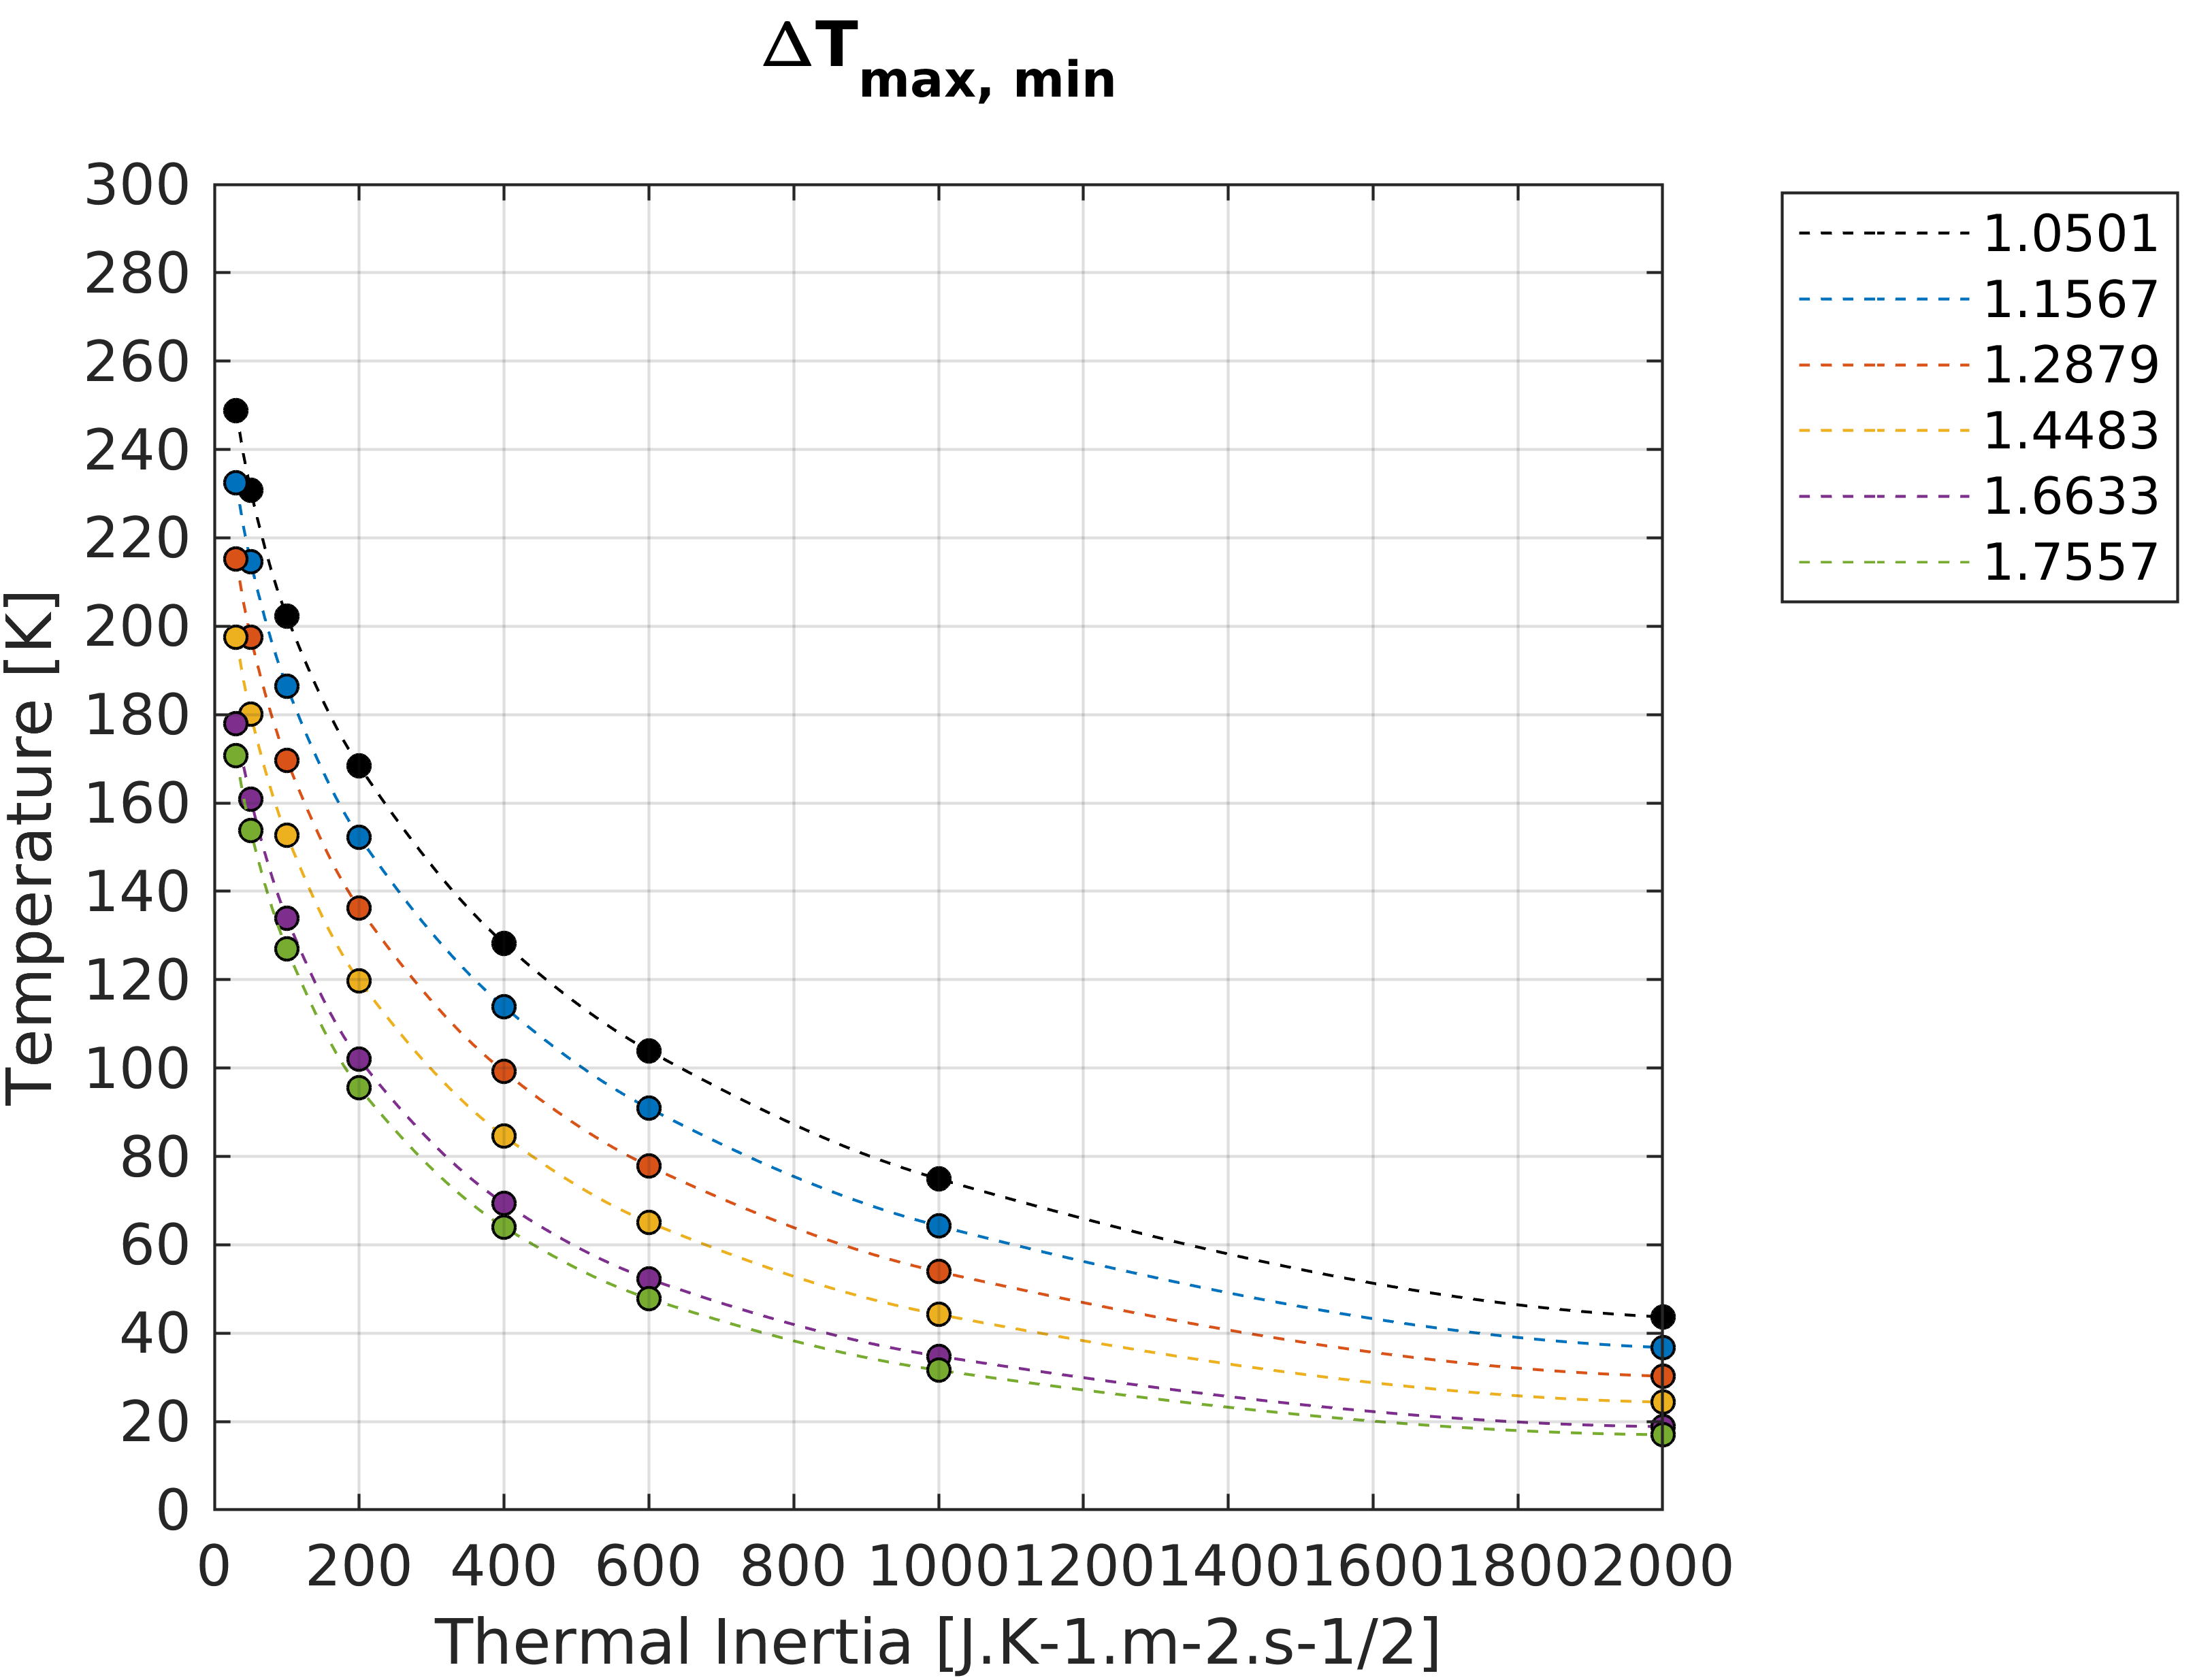
\includegraphics[width=0.49\linewidth]{rsc/temp_gammas_delta.png}
    \captionof{figure}{Influence of the thermal intertia on the maximum variations of the daily surface temperatures. Simulation in the first figure is for an heliocentric distance of 1.0501 AU. The second image shows the difference between the maximum and the minimum temperature for several distances.}
    \label{fig:8.3}
\end{figure*}
